

\tikzset{every picture/.style={line width=0.75pt}} %set default line width to 0.75pt

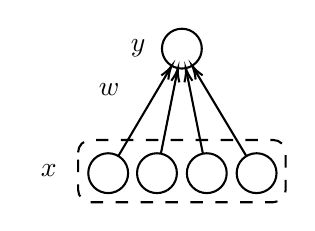
\begin{tikzpicture}[x=0.75pt,y=0.75pt,yscale=-1,xscale=1]
%uncomment if require: \path (0,146); %set diagram left start at 0, and has height of 146

%Rounded Rect [id:dp492723450593467]
\draw  [dash pattern={on 4.5pt off 4.5pt}] (120,86) .. controls (120,82.69) and (122.69,80) .. (126,80) -- (214,80) .. controls (217.31,80) and (220,82.69) .. (220,86) -- (220,104) .. controls (220,107.31) and (217.31,110) .. (214,110) -- (126,110) .. controls (122.69,110) and (120,107.31) .. (120,104) -- cycle ;

% Text Node
\draw    (134.5, 96) circle [x radius= 9.6, y radius= 9.6]   ;
\draw (134.5,96) node   [align=left] {\begin{minipage}[lt]{8.67pt}\setlength\topsep{0pt}

\end{minipage}};
% Text Node
\draw    (158, 96) circle [x radius= 9.6, y radius= 9.6]   ;
\draw (158,96) node   [align=left] {\begin{minipage}[lt]{8.67pt}\setlength\topsep{0pt}

\end{minipage}};
% Text Node
\draw    (182, 96) circle [x radius= 9.6, y radius= 9.6]   ;
\draw (182,96) node   [align=left] {\begin{minipage}[lt]{8.67pt}\setlength\topsep{0pt}

\end{minipage}};
% Text Node
\draw    (206, 96) circle [x radius= 9.6, y radius= 9.6]   ;
\draw (206,96) node   [align=left] {\begin{minipage}[lt]{8.67pt}\setlength\topsep{0pt}

\end{minipage}};
% Text Node
\draw    (170, 36) circle [x radius= 9.6, y radius= 9.6]   ;
\draw (170,36) node   [align=left] {\begin{minipage}[lt]{8.67pt}\setlength\topsep{0pt}

\end{minipage}};
% Text Node
\draw (105.93,95) node   [align=left] {\begin{minipage}[lt]{8.67pt}\setlength\topsep{0pt}
\begin{center}
$\displaystyle \boldsymbol{x}$
\end{center}

\end{minipage}};
% Text Node
\draw (134.93,56) node   [align=left] {\begin{minipage}[lt]{8.67pt}\setlength\topsep{0pt}
\begin{center}
$\displaystyle \boldsymbol{w}$
\end{center}

\end{minipage}};
% Text Node
\draw (148.93,36) node   [align=left] {\begin{minipage}[lt]{8.67pt}\setlength\topsep{0pt}
\begin{center}
$\displaystyle y$
\end{center}

\end{minipage}};
% Connection
\draw    (139.39,87.73) -- (164.09,45.99) ;
\draw [shift={(165.11,44.27)}, rotate = 480.61] [color={rgb, 255:red, 0; green, 0; blue, 0 }  ][line width=0.75]    (6.56,-1.97) .. controls (4.17,-0.84) and (1.99,-0.18) .. (0,0) .. controls (1.99,0.18) and (4.17,0.84) .. (6.56,1.97)   ;
% Connection
\draw    (159.88,86.58) -- (167.72,47.38) ;
\draw [shift={(168.12,45.42)}, rotate = 461.31] [color={rgb, 255:red, 0; green, 0; blue, 0 }  ][line width=0.75]    (6.56,-1.97) .. controls (4.17,-0.84) and (1.99,-0.18) .. (0,0) .. controls (1.99,0.18) and (4.17,0.84) .. (6.56,1.97)   ;
% Connection
\draw    (180.12,86.58) -- (172.28,47.38) ;
\draw [shift={(171.88,45.42)}, rotate = 438.69] [color={rgb, 255:red, 0; green, 0; blue, 0 }  ][line width=0.75]    (6.56,-1.97) .. controls (4.17,-0.84) and (1.99,-0.18) .. (0,0) .. controls (1.99,0.18) and (4.17,0.84) .. (6.56,1.97)   ;
% Connection
\draw    (201.06,87.76) -- (175.97,45.95) ;
\draw [shift={(174.94,44.24)}, rotate = 419.03999999999996] [color={rgb, 255:red, 0; green, 0; blue, 0 }  ][line width=0.75]    (6.56,-1.97) .. controls (4.17,-0.84) and (1.99,-0.18) .. (0,0) .. controls (1.99,0.18) and (4.17,0.84) .. (6.56,1.97)   ;

\end{tikzpicture}